\myheader{Guía 3: Series de Fourier}

\begin{ejercicio}
    Obtener la representación en serie de Fourier de tiempo continuo de las siguientes señales de tiempo continuo y determinar su período fundamental:
    \begin{align*}
        \inciso & 1 + e^{j\frac{\pi}{4}t} + 4e^{-j\frac{2\pi}{5}t} + e^{j\frac{4\pi}{5}t} &
        \inciso & 2 + \cos\left(\frac{2\pi}{3}t\right) + 3\sin\left(\frac{5\pi}{3}t\right)
    \end{align*}
\end{ejercicio}

\begin{ejercicio}
    Una señal periódica $x(t)$ real de tiempo continuo tiene período $T=8$ y sus coeficientes de la serie de Fourier no nulos son:
    \begin{equation*}
        a_1 = a_{-1} = 2, a_3 = { }^* a_{-3} = 4j
    \end{equation*}
    Hallar $A_k, \phi_k$ con $k\in \Z$ de manera que el desarrollo en serie de Fourier de $x(t)$ puede ser expresado como
    \begin{equation*}
        x(t) = \sum_{k=0}^{\infty} A_k \cos\left(\frac{2\pi}{T}t + \phi_k\right)
    \end{equation*}
\end{ejercicio}

\begin{ejercicio}
Sea $x(t)$ un tren de pulsos de período $T$ definido en el intervalo $[-\frac{T}{2},\frac{T}{2})$ como 
\begin{equation*}
    x(t) = \begin{cases}
    1 & \mbox{si } t \in (-\frac{T_0}{2},\frac{T_0}{2}) \\
    0 & \mbox{si } t \in [-\frac{T}{2},-\frac{T_0}{2}) \cup (\frac{T_0}{2},\frac{T}{2})
    \end{cases}
\end{equation*}
\end{ejercicio}
con $T > T_0 > 0$. 

\inciso Calcular utilizando la ecuación de síntesis los coeficientes $\left\{a_k\right\}_{k\in\mathbb{Z}}$ de la Serie de Fourier de tiempo continuo de $x(t)$ y escriba los 6 primeros términos de la serie.

\inciso Graficar el espectro de amplitudes y de fase.

\inciso Obtener los coeficientes $\left\{b_k\right\}_{k\in\mathbb{Z}}$ de la Serie de Fourier de tiempo continuo de $x_1(t) = x(t-\frac{\pi}{6})$.

\inciso Obtener los coeficientes $\left\{c_k\right\}_{k\in\mathbb{Z}}$ de la Serie de Fourier de tiempo continuo de $x_2(t) = x(t)+1$.

\inciso Calcular utilizando la ecuación de síntesis la representación en serie de Fourier de un tren de impulsos de período $T$ y obtener los coeficientes $\left\{a_k\right\}_{k\in\mathbb{Z}}$ de la Serie de Fourier de tiempo continuo de $x(t)$ a partir de la combinación de dos trenes de impulsos de período $T$ desplazados.

\begin{ejercicio}
Utilizando las propiedades de la serie de Fourier de tiempo continuo, calcular los coeficientes $\left\{a_k\right\}_{k\in\mathbb{Z}}$ de la señal periódica $x(t)$. 
\begin{align*}
    \inciso & \parbox{.4\textwidth}{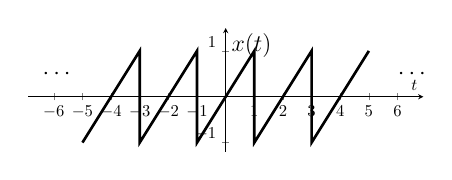
\begin{tikzpicture}[scale=0.6]
    \begin{axis}[
        x=.05\textwidth,y=0.08\textwidth,
    	axis y line=center,
    	axis x line=middle,
    	xlabel=$t$,ylabel={\Large $x(t)$},
    	xmin=-6.9,xmax=6.9,
    	ymin=-1.2,ymax=1.5,
    	xtick={-6,...,6},
    	xticklabel style = {xshift=0},
    	yticklabel style = {yshift=5}
	] 
	\addplot[
    	black,
    	ultra thick
    	] coordinates {
	(-5,-1) (-3,1) (-3,-1) (-1,1) (-1,-1) (1,1) (1,-1) (3,1) (3,-1) (5,1)
	} ;
	\node at (axis cs:6.5,0.5) {\Large $\cdots$} ;
	\node at (axis cs:-5.9,0.5) {\Large $\cdots$} ;
    \end{axis}
\end{tikzpicture}} & \hspace{\fill} 
    \inciso & \parbox{.4\textwidth}{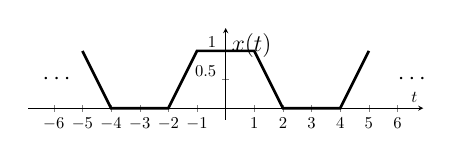
\begin{tikzpicture}[scale=0.6]
    \begin{axis}[
        x=.05\textwidth,y=0.1\textwidth,
    	axis y line=center,
    	axis x line=middle,
    	xlabel=$t$,ylabel={\Large $x(t)$},
    	xmin=-6.9,xmax=6.9,
    	ymin=-0.2,ymax=1.4,
    	xtick={-6,...,6},
    	xticklabel style = {xshift=0},
    	yticklabel style = {yshift=5}
	] 
	\addplot[
    	black,
    	ultra thick
    	] coordinates {
	(-5, 1) (-4, 0) (-2,0) (-1,1) (1,1) (2,0) (4,0) (5,1)
	} ;
	\node at (axis cs:6.5,0.5) {\Large $\cdots$} ;
	\node at (axis cs:-5.9,0.5) {\Large $\cdots$} ;
    \end{axis}
\end{tikzpicture}} \\
    \inciso & \parbox{.4\textwidth}{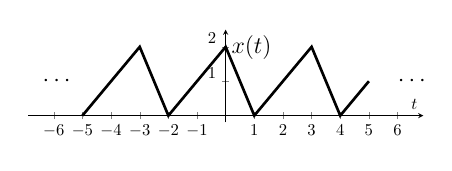
\begin{tikzpicture}[scale=0.6]
    \begin{axis}[
        x=.05\textwidth,y=0.06\textwidth,
    	axis y line=center,
    	axis x line=middle,
    	xlabel=$t$,ylabel={\Large $x(t)$},
    	xmin=-6.9,xmax=6.9,
    	ymin=-0.2,ymax=2.5,
    	xtick={-6,...,6},
    	xticklabel style = {xshift=0},
    	yticklabel style = {yshift=5}
	] 
	\addplot[
    	black,
    	ultra thick
    	] coordinates {
	(-5,0) (-3,2) (-2,0) (0,2) (1,0) (3,2)
	(4,0) (5,1)
	} ;
	\node at (axis cs:6.5,1) {\Large $\cdots$} ;
	\node at (axis cs:-5.9,1) {\Large $\cdots$} ;
    \end{axis}
\end{tikzpicture}} & \hspace{\fill} 
    \inciso & \parbox{.4\textwidth}{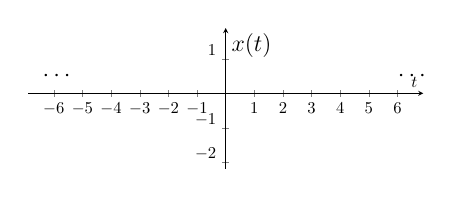
\begin{tikzpicture}[scale=0.6]
    \begin{axis}[
        x=.05\textwidth,y=0.06\textwidth,
    	axis y line=center,
    	axis x line=middle,
    	xlabel=$t$,ylabel={\Large $x(t)$},
    	xmin=-6.9,xmax=6.9,
    	ymin=-2.2,ymax=1.9,
    	xtick={-6,...,6},
    	xticklabel style = {xshift=0},
    	yticklabel style = {yshift=5}
	] 
	\diracdelta{-5}{-2};
	\diracdelta{-4}{1};
	\diracdelta{-3}{-2};
	\diracdelta{-2}{1};
	\diracdelta{-1}{-2};
	\diracdelta{0}{1};
	\diracdelta{1}{-2};
	\diracdelta{2}{1};
	\diracdelta{3}{-2};
	\diracdelta{4}{1};
	\diracdelta{5}{-2};
	\node at (axis cs:6.5,.5) {\Large $\cdots$} ;
	\node at (axis cs:-5.9,.5) {\Large $\cdots$} ;
    \end{axis}
\end{tikzpicture}} \\
    \inciso & \parbox{.4\textwidth}{\input{03_series_fourier/plots/3-2e}} & \hspace{\fill} 
    \inciso & \parbox{.4\textwidth}{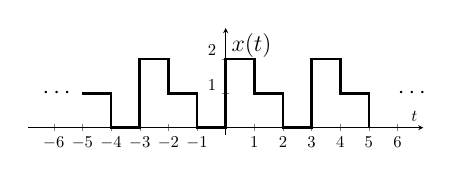
\begin{tikzpicture}[scale=0.6]
    \begin{axis}[
        x=.05\textwidth,y=0.06\textwidth,
    	axis y line=center,
    	axis x line=middle,
    	xlabel=$t$,ylabel={\Large $x(t)$},
    	xmin=-6.9,xmax=6.9,
    	ymin=-0.2,ymax=2.9,
    	xtick={-6,...,6},
    	xticklabel style = {xshift=0},
    	yticklabel style = {yshift=5}
	] 
	\addplot[
    	black,
    	ultra thick
    	] coordinates {
	(-5,1) (-4,1) (-4,0) (-3,0) (-3,2) (-2,2) (-2,1) (-1,1) (-1,0) (0,0) (0,2) (1,2) (1,1) (2,1) (2,0) (3,0) (3,2) (4,2) (4,1) (5,1) (5,0)
	} ;
	\node at (axis cs:6.5,1) {\Large $\cdots$} ;
	\node at (axis cs:-5.9,1) {\Large $\cdots$} ;
    \end{axis}
\end{tikzpicture}} \\
    \inciso & \parbox{.4\textwidth}{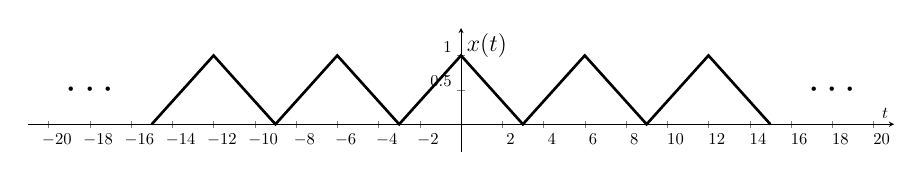
\begin{tikzpicture}[scale=0.6,transform shape]
    \begin{axis}[
        x=0.036\textwidth,y=0.12\textwidth,
    	axis y line=center,
    	axis x line=middle,
    	xlabel=$t$,ylabel={\Large $x(t)$},
    	xmin=-21,xmax=21,
    	ymin=-0.4,ymax=1.4,
    	xticklabel style = {xshift=5},
    	yticklabel style = {yshift=5},
    	]
    	\addplot[
    	black,
    	ultra thick
    	] coordinates {
    	    (-15,0) (-12,1) 
    	    (-9,0) (-6,1)
    	    (-3,0) (0,1)
    	    (3,0) (6,1)
    	    (9,0) (12,1)
    	    (15,0)
    	};
    	\node at (18,0.5) {\Huge $\cdots$} ;
    	\node at (-18,0.5) {\Huge $\cdots$} ;
    \end{axis}
\end{tikzpicture}} & \hspace{\fill} & \\
\end{align*}
\end{ejercicio}

\begin{ejercicio}
Calcular los coeficientes de la serie de Fourier de tiempo continuo de la señal $x(t)$ de período $T=3$ sabiendo que en el intervalo $[-1.5,1.5)$ se define como

\inciso $x(t) = \cos(20\pi t)w_1(t)$ con \begin{equation*}
    w_1(t) = \begin{cases}
    1 & \mbox{si } t \in (-1,1) \\
    0 & \mbox{si } t \in [-1.5,\,-1) \cup (1,1.5)
    \end{cases}
\end{equation*}

\inciso $x(t) = \cos(20\pi t)w_2(t)$ con \begin{equation*}
    w_2(t) = \begin{cases}
    1 & \mbox{si } t \in (-1.5,-1) \\
    0 & \mbox{si } t \in [-1,0) \\
    2 & \mbox{si } t \in (0,1) \\
    1 & \mbox{si } t \in (1,1.5) \\
    \end{cases}
\end{equation*}

\inciso $x(t) = \cos(20\pi t)w_3(t)$ con \begin{equation*}
    w_3(t) = \begin{cases}
    e^{-|t|} & \mbox{si } t \in (-1,1) \\
    0 & \mbox{si } t \in [-1.5,-1) \cup (1,1.5)
    \end{cases}
\end{equation*}
\end{ejercicio}


\begin{ejercicio}
    Obtener dos señales de tiempo continuo que satisfagan simultáneamente las siguientes condiciones:
    \begin{enumerate}
        \item $x(t)$ es real e impar.
        \item $x(t)$ es periódica con período $T=2$.
        \item Los coeficientes de Fourier de $x(t)$ son $\{a_k\}_{k \in \Z}$ con $a_k = 0, |k| > 1$.
        \item $\frac{1}{2} \int_{0}^{2} |x(t)|^2 \, dt = 1$.
    \end{enumerate}
\end{ejercicio}

\begin{ejercicio}
    Sea $x(n)$ una señal discreta real e impar de período $N=7$ y coeficientes de Fourier $\{a_k\}_{k \in \Z}$. Dado que se sabe que:
    \begin{equation*}
        a_{15} = j, a_{16} = 2j, a_{17} = 3j
    \end{equation*}
    determinar los valores de $a_0,a_{-1},a_{-2}$ y $a_{-3}$.
\end{ejercicio}

\begin{ejercicio}
Utilizando las propiedades de la serie de Fourier de tiempo discreto, calcular los coeficientes $\left\{a_k\right\}_{k=0}^{N}$ de la señal periódica $x(n)$:
\begin{align*}
    \inciso & \parbox{.4\textwidth}{\input{03_series_fourier/plots/3-dtft_a}} & \hspace{\fill} 
    \inciso & \parbox{.4\textwidth}{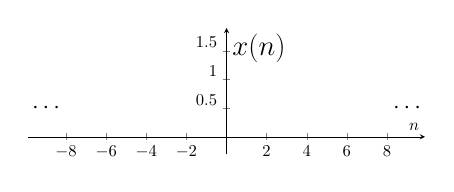
\begin{tikzpicture}[scale=0.6,transform shape]
    \begin{axis}[
        x=0.035\textwidth,y=0.1\textwidth,
    	axis y line=center,
    	axis x line=middle,
    	xlabel=$n$,ylabel={\LARGE $x(n)$},
    	xmin=-9.9,xmax=9.9,
    	ymin=-0.3,ymax=1.9,
    	xticklabel style = {xshift=0},
    	yticklabel style = {yshift=5},
    	]
    	\discretedelta{-8}{0.1};
    	\discretedelta{-7}{0.1};
    	\discretedelta{-6}{1};
    	\discretedelta{-5}{1};
    	\discretedelta{-4}{1};
    	\discretedelta{-3}{1};
    	\discretedelta{-2}{0.1};
    	\discretedelta{-1}{0.1};
    	\discretedelta{0}{1};
    	\discretedelta{1}{1};
    	\discretedelta{2}{1};
    	\discretedelta{3}{1};
    	\discretedelta{4}{0.1};
    	\discretedelta{5}{0.1};
    	\discretedelta{6}{1};
    	\discretedelta{7}{1};
    	\discretedelta{8}{1};
    	\node at (-9,0.5) {\Large $\cdots$};
    	\node at (9,0.5) {\Large $\cdots$};
    \end{axis}
\end{tikzpicture}} \\
    \inciso & \parbox{.4\textwidth}{\begin{tikzpicture}[scale=0.6,transform shape]
    \begin{axis}[
        x=0.035\textwidth,y=0.08\textwidth,
    	axis y line=center,
    	axis x line=middle,
    	xlabel=$n$,ylabel={\LARGE $x(n)$},
    	xmin=-9.9,xmax=9.9,
    	ymin=-1.4,ymax=2.9,
    	xticklabel style = {xshift=0},
    	yticklabel style = {yshift=5},
    	]
    	\discretedelta{-8}{-1};
    	\discretedelta{-7}{2};
    	\discretedelta{-6}{1};
    	\discretedelta{-5}{2};
    	\discretedelta{-4}{-1};
    	\discretedelta{-3}{0.1};
    	\discretedelta{-2}{-1};
    	\discretedelta{-1}{2};
    	\discretedelta{0}{1};
    	\discretedelta{1}{2};
    	\discretedelta{2}{-1};
    	\discretedelta{3}{0.1};
    	\discretedelta{4}{-1};
    	\discretedelta{5}{2};
    	\discretedelta{6}{1};
    	\discretedelta{7}{2};
    	\discretedelta{8}{-1};
    	\node at (-9,0.5) {\Large $\cdots$};
    	\node at (9,0.5) {\Large $\cdots$};
    \end{axis}
\end{tikzpicture}} & \hspace{\fill} 
    \inciso & x(n) = \sin(2\pi n / 3) \cos(\pi n/2)
\end{align*}

\noindent \hspace*{0.6em} \inciso $x(n)$ periódica con período 4, siendo $x(n) = 1-\sin(\pi n/4)$ para $0 \leq n \leq 3$ 

\noindent \hspace*{0.6em} \inciso $x(n)$ periódica con período 12, siendo $x(n) = 1-\sin(\pi n/4)$ para $0 \leq n \leq 11$
\end{ejercicio}

\begin{ejercicio}
Sea $x(n)$ una señal periódica de período $N$, con sus coeficientes de serie de Fourier $\{a_k\}_{k\in \Z}$. Hallar los coeficientes de las siguientes señales periódicas de período $N$:
\begin{align*}
    & \inciso x(n-n_0),\; n_0 \in\mathbb{Z} & \hfill & \inciso x(n) - x(n-1) & \hfill & \inciso x(n) - x\left(n-\frac{N}{2}\right),\; \mbox{$N$ par} \\
    & \inciso x(n) + x\left(n-\frac{N}{2}\right),\; \mbox{$N$ par} & \hfill & \inciso x^*(-n) & \hfill & \inciso (-1)^n x(n),\; \mbox{$N$ par} \\ & \inciso (-1)^n x(n),\; \mbox{$N$ impar}
    & \hfill & \inciso y(n) = \begin{cases} x(n) & \mbox{si $n$ es par} \\ 0 & \mbox{en otro caso}
    \end{cases}
\end{align*}
\end{ejercicio}

\begin{ejercicio}
Sea un sistema LTI de tiempo continuo con respuesta al impulso $h(t) = e^{-4|t|}$. Hallar la salida $y(t)$ del sistema para las siguientes entradas:

\inciso $x(t)=e^{j\omega_0 t}$ con $\omega_0\in\mathbb{R}$ ¿Es $x(t)$ una autofunción del sistema?

\inciso $x(t)=e^{j\omega_0 t}u(t)$ con $\omega_0\in\mathbb{R}$. ¿Es $x(t)$ una autofunción del sistema?

\inciso $x(t)=\sum_{k=-\infty}^{\infty} (-1)^k \delta(t-k)$

\inciso $x(t)$ de período 1 tal que $x(t) = \begin{cases} 1 & \mbox{si $-1/4 \leq t < 1/4$} \\ 0 & \mbox{en otro caso} \end{cases}$ \hspace{1em} para $-1/2\leq t < 1/2$.
\end{ejercicio}

\begin{ejercicio}
    Sea el sistema LTI de tiempo discreto cuya respuesta en frecuencia es:
    \begin{equation*}
        H(e^{j\omega}) = \begin{cases}
            1 & \mbox{si $|\omega| \leq \frac{\pi}{8}$} \\
            0 & \mbox{si } \frac{\pi}{8} < |\omega| \leq \pi \\
        \end{cases}
    \end{equation*}
    Mostrar que si la entrada $x(n)$ al sistema tiene período $N=3$, entonces la salida $y(n)$ tiene un único valor no nulo por período. 
\end{ejercicio}

\begin{ejercicio}
Para cada uno de los siguientes pares de señales $x(n)$ e $y(n)$, determinar si existe un sistema LTI discreto cuya salida $y(n)$ pueda corresponder efectivamente a la entrada $x(n)$. En el caso de que exista, determinar si es único y qué codiciones debe cumplir la respuesta al impulso.

\inciso $x(n) = \left(\frac{1}{2}\right)^n$ e $y(n) = \left(\frac{1}{4}\right)^n$

\inciso $x(n)=e^{jn/8}$ e $y(n) = e^{j2n/8}$

\inciso $x(n)= e^{j\pi n/3}$ e $y(n) = \cos(\pi n/3)$

\inciso $x(n) = \cos(\pi n/3)$ e $y(n) = \cos(\pi n/3) + \sqrt{3} \sin(\pi n/3)$
\end{ejercicio}

\begin{ejercicio}
Decidir si existe un sistema LTI discreto que cumpla con que si $x(n)$ es la entrada, entonces $y(n)$ es una salida posible.
\begin{align*}
    \inciso & \parbox{.4\textwidth}{
        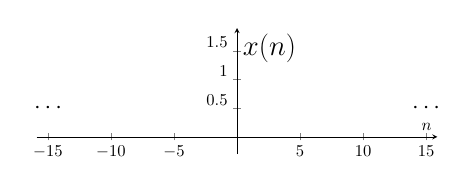
\begin{tikzpicture}[scale=0.6,transform shape]
    \begin{axis}[
        x=0.022\textwidth,y=0.1\textwidth,
    	axis y line=center,
    	axis x line=middle,
    	xlabel=$n$,ylabel={\LARGE $x(n)$},
    	xmin=-15.9,xmax=15.9,
    	ymin=-0.3,ymax=1.9,
    	xticklabel style = {xshift=0},
    	yticklabel style = {yshift=5}
    	]
    	\discretedelta{-14}{0.1};
    	\discretedelta{-13}{1};
    	\discretedelta{-12}{1};
    	\discretedelta{-11}{1};
    	\discretedelta{-10}{0.1};
    	\discretedelta{-9}{0.1};
    	\discretedelta{-8}{0.1};
    	\discretedelta{-7}{0.1};
    	\discretedelta{-6}{0.1};
    	\discretedelta{-5}{0.1};
    	\discretedelta{-4}{0.1};
    	\discretedelta{-3}{0.1};
    	\discretedelta{-2}{0.1};
    	\discretedelta{-1}{1};
    	\discretedelta{0}{1};
    	\discretedelta{1}{1};
    	\discretedelta{2}{0.1};
    	\discretedelta{3}{0.1};
    	\discretedelta{4}{0.1};
    	\discretedelta{5}{0.1};
    	\discretedelta{6}{0.1};
    	\discretedelta{7}{0.1};
    	\discretedelta{8}{0.1};
    	\discretedelta{9}{0.1};
    	\discretedelta{10}{0.1};
    	\discretedelta{11}{1};
    	\discretedelta{12}{1};
    	\discretedelta{13}{1};
    	\discretedelta{14}{0.1};
    	\node at (-15,0.5) {\Large $\cdots$};
    	\node at (15,0.5) {\Large $\cdots$};
    \end{axis}
\end{tikzpicture}
    } 
    & \hspace{\fill} 
    & \parbox{.4\textwidth}{
        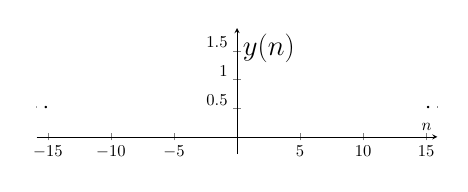
\begin{tikzpicture}[scale=0.6,transform shape]
    \begin{axis}[
        x=0.022\textwidth,y=0.1\textwidth,
    	axis y line=center,
    	axis x line=middle,
    	xlabel=$n$,ylabel={\LARGE $y(n)$},
    	xmin=-15.9,xmax=15.9,
    	ymin=-0.3,ymax=1.9,
    	xticklabel style = {xshift=0},
    	yticklabel style = {yshift=5}
    	]
    	\discretedelta{-14}{1};
    	\discretedelta{-13}{0.1};
    	\discretedelta{-12}{0.1};
    	\discretedelta{-11}{0.1};
    	\discretedelta{-10}{1};
    	\discretedelta{-9}{1};
    	\discretedelta{-8}{1};
    	\discretedelta{-7}{0.1};
    	\discretedelta{-6}{0.1};
    	\discretedelta{-5}{0.1};
    	\discretedelta{-4}{1};
    	\discretedelta{-3}{1};
    	\discretedelta{-2}{1};
    	\discretedelta{-1}{0.1};
    	\discretedelta{0}{0.1};
    	\discretedelta{1}{0.1};
    	\discretedelta{2}{1};
    	\discretedelta{3}{1};
    	\discretedelta{4}{1};
    	\discretedelta{5}{0.1};
    	\discretedelta{6}{0.1};
    	\discretedelta{7}{0.1};
    	\discretedelta{8}{1};
    	\discretedelta{9}{1};
    	\discretedelta{10}{1};
    	\discretedelta{11}{0.1};
    	\discretedelta{12}{0.1};
    	\discretedelta{13}{0.1};
    	\discretedelta{14}{1};
    	\node at (-16,0.5) {\Large $\cdots$};
    	\node at (16,0.5) {\Large $\cdots$};
    \end{axis}
\end{tikzpicture}
    } \\
    \inciso & \parbox{.4\textwidth}{
        \input{03_series_fourier/plots/3-eigenfunction_b}
    } & \hspace{\fill} 
    & \parbox{.4\textwidth}{
        \input{03_series_fourier/plots/3-eigenfunction_bb}
    }
\end{align*}
En caso de que se cumpla, decidir si es posible asegurar que todos los sistemas que cumplan con esta condición son realmente LTI.
\end{ejercicio}

\begin{ejercicio}
    Cuando un tren de impulsos
    \begin{equation*}
        x(n) = \sum_{k=-\infty}^{\infty} \delta(n-4k)
    \end{equation*}
    pasa por un sistema LTI con una respuesta en frecuencia $H\left(e^{j\omega}\right)$, la salida es
    \begin{equation*}
        y(n) = \cos\left(\frac{5\pi}{2}n + \frac{\pi}{4}\right)
    \end{equation*}
    Determinar el valor de $H\left(e^{j\frac{k\pi}{2}}\right)$ para $k=0,1,2,3$.
\end{ejercicio}

\begin{ejercicio}
    Sea un sistema LTI de tiempo discreto cuya respuesta al impulso vale 
    \begin{equation*}
        h(n) = \frac{\sin\left(\frac{3\pi n}{10}\right)}{\sin\left(\frac{\pi n}{10}\right)},\; n = 0,\ldots, 9
    \end{equation*}
    y cero en otro caso.

    \inciso Se considera la entrada al sistema que vale
    \begin{equation*}
        x_1(n) = \frac{\sin\left(\frac{7\pi n}{10}\right)}{\sin\left(\frac{\pi n}{10}\right)}, \; n = 0,\ldots, 9
    \end{equation*}
    y cero en otro caso. A su vez, se considera la señal $\tilde{y}(n)$ que corresponde a la periodización (con período 10) de la salida $y(n)$ a la entrada $x_1(n)$. Determinar $\tilde{y}(n)$.

    \inciso Determinar la salida del sistema descripto por $h(n)$ cuando la entrada vale 
    \begin{equation*}
        x_2(n) = \cos\left(\frac{6\pi n}{10}\right), \; \mbox{para todo $n$}
    \end{equation*}
\end{ejercicio}